% Robot <-> laptop packet diagram. Two curved messages, each with a
% colored header and white body in a single cell.

\documentclass[border=10pt]{standalone}
\usepackage{tikz}
\usepackage{lmodern}
\usepackage[T1]{fontenc}
\usepackage{xcolor}
\pagecolor{white}
\usetikzlibrary{positioning,calc,arrows.meta,shapes.multipart,backgrounds}

\definecolor{hostcolor}{HTML}{1F4E79}
\definecolor{robotcolor}{HTML}{A03028}
\definecolor{endpointfill}{HTML}{F4F1EA}

\begin{document}
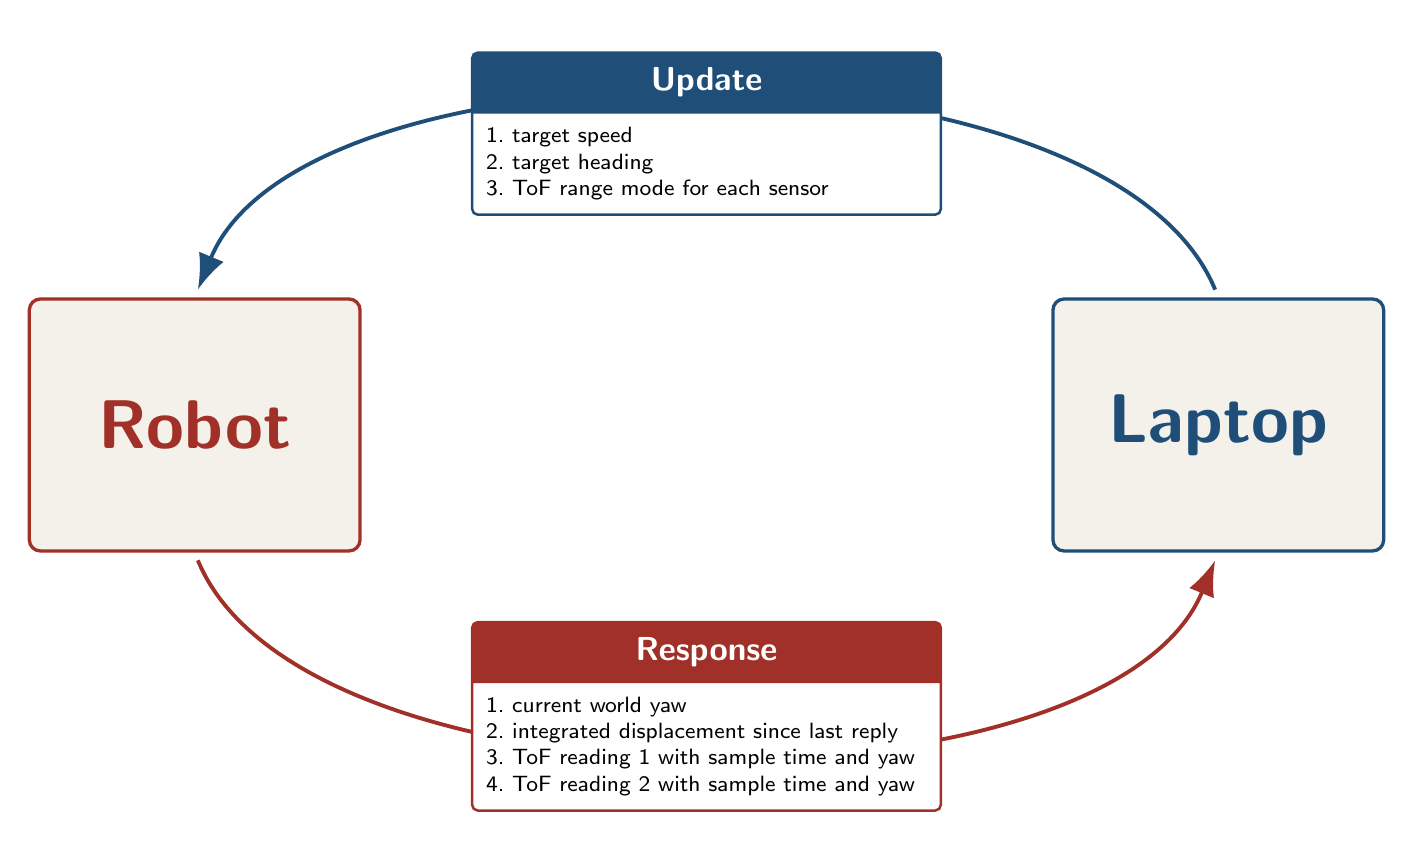
\begin{tikzpicture}[
  font=\sffamily,
  >={Latex[length=4.5mm,width=3.4mm]},
  endpoint/.style 2 args={
    draw=#1, fill=endpointfill, line width=1.2pt,
    rounded corners=4pt,
    minimum width=4.2cm, minimum height=3.2cm,
    align=center,
    font=\sffamily\bfseries\Huge, text=#1,
  },
  msgarrow/.style={->, line width=1.4pt, color=#1, shorten >=3pt, shorten <=3pt},
  msgcell/.style 2 args={
    rectangle split, rectangle split parts=2,
    rectangle split part fill={#1, white},
    draw=#1, line width=0.9pt, rounded corners=2pt,
    text width=#2, align=center,
    font=\sffamily\footnotesize, text=black,
    inner sep=5pt,
  },
]

% --- endpoints ------------------------------------------------------
\node[endpoint={robotcolor}{}] (R) at (0,0)  {Robot};
\node[endpoint={hostcolor}{}]  (L) at (13,0) {Laptop};

\def\msgw{5.6cm}

% --- update (laptop -> robot, arc over the top) --------------------
\node[msgcell={hostcolor}{\msgw}] (U) at (6.5,3.7) {%
  {\color{white}\bfseries\large Update}
  \nodepart[align=left]{two}%
    1.\ target speed\\
    2.\ target heading\\
    3.\ ToF range mode for each sensor
};

\begin{scope}[on background layer]
  \draw[msgarrow=hostcolor]
    (L.north)
      .. controls ($(L.north)+(-1.4,3.4)$)
      and        ($(R.north)+( 1.4,3.4)$) ..
    (R.north);
\end{scope}

% --- response (robot -> laptop, arc under the bottom) ---------------
\node[msgcell={robotcolor}{\msgw}] (D) at (6.5,-3.7) {%
  {\color{white}\bfseries\large Response}
  \nodepart[align=left]{two}%
    1.\ current world yaw\\
    2.\ integrated displacement since last reply\\
    3.\ ToF reading 1 with sample time and yaw\\
    4.\ ToF reading 2 with sample time and yaw
};

\begin{scope}[on background layer]
  \draw[msgarrow=robotcolor]
    (R.south)
      .. controls ($(R.south)+( 1.4,-3.4)$)
      and        ($(L.south)+(-1.4,-3.4)$) ..
    (L.south);
\end{scope}

\end{tikzpicture}
\end{document}
